\documentclass{article}

\usepackage[utf8]{inputenc}
\usepackage[T1]{fontenc}
\usepackage{lipsum}
\usepackage{graphicx}
\usepackage{amsmath}
\usepackage[margin=1in]{geometry}
\usepackage{titlesec}
\usepackage{enumitem}

\titleformat{\section}
{\LARGE\bfseries}{\thesection}{1em}{}

\titleformat{\subsection}
{\Large\bfseries}{\thesection}{1em}{}

\begin{document}

\pagestyle{empty}

\section*{HW2}
\large

\subsection*{Traccia}
\large
Una \textbf{università} è strutturata in \textbf{scuole} e \textbf{dipartimenti}. Le scuole raggruppano vari \textbf{corsi di studio}. I corsi di studio sono strutturati in annualità compredenti vari \textbf{insegnamenti}. Gli insegnamenti vengono tenuti da un \textbf{docente}, che riferisce a un \textbf{dipartimento}. Gli \textbf{studenti} si iscrivono ad una \textbf{annualità} di un corso di studio ed hanno un \textbf{piano di studio} per quell'anno formato dagli \textbf{insegnamenti} fondamentali previsti dal corso più altri che loro scelgono fra i \textbf{fondamentali} di altri corsi o fra gli insegnamenti \textbf{complementari}. Nel piano di studio possono essere presenti anche attività di \textbf{tirocinio} e/o la \textbf{prova finale}. L'\textbf{iscrizione} di uno studente è attiva per un periodo di tempo definito; una volta scaduta deve essere rinnovata per l'annualità successiva o per la stessa annualità. Si tracci un diagramma di dominio rappresentante la realtà descritta.

\subsubsection*{Risoluzione}
\large
\textit{Individuazione delle classi - regole utili}\\
In un esercizio simile occorre che sia individuata la totalità delle classi e ciò avviene mediante l'analisi di tutti i \textit{sostantivi} presenti nella traccia. Per cui il primo passo consiste proprio nel marcare tutto ciò che possa essere considerato un sostantivo, in grado di poter compiere un'azione; infatti come da traccia sono stati evidenziati in grassetto tutti gli elementi che possano poi costituire le differenti classi.\vspace*{14pt}\\
La fase successiva prevede una \textit{scrematura} dei sinonimi, ossia di sostantivi di etimologia e di senso simile che possano compiere medesimi comportamenti.\\
Infine l'ultimo step prevede la rappresentazione del digramma dei domini (\textit{a.k.a diagramma della classi}), ponendo particolare attenzione alle associazioni usate, alle cardinalità espresse e creare i corretti collegamenti che permettano di risalire a tutte le possibili informazioni richieste.
\subsubsection*{Considerazioni}
\textit{Precedenti alla correzione}\\
Il diagramma propone la \textit{totalità} dei sostantivi evidenziati, dato che nessun sinonimo, a livello di etimologia e senso, compia effettivamente delle azioni ridondanti.\\
Sono abbinate un buon numero di associazioni, come la \textit{composizione} e l'\textit{aggregazione}, le quali risultano essere correttamente poste, anche se in relazione ad alcune connessioni non sarebbe possibile risalire a certe informazioni; un esempio è proprio dato dallo \textit{Studente} e dal \textit{Piano di studio}, in cui sarebbe difficile ottenere dati interpretabili. Questo è dovuto principalmente alle cardinalità; infatti, in un modello simile, le molteplicità (\textit{a molti}), indicate con il simbolo \textit{*}, non permettono in questo contesto di poter acquisire informazioni in maniera diretta di un piano di studio per un unico studente. Per cui, concludendo, sarebbe stato conveniente porre un'\textit{associazione} tra le classi \textit{Studente} e \textit{Piano di studio}.\\
Ultima considerazione è inerente all'uso dell'\textit{ereditarietà}, la quale si osserva tra le classi \textit{Insegnamento}, \textit{Obbligatorio} e \textit{Opzionale}. Non è un errore conciso, ma non rappresenta nemmeno un buon metodo per esprimere che un \textit{Insegnamento} possa essere \textit{Opzionale} oppure \textit{Obbligatorio}.
\pagebreak
\subsubsection*{Diagramma delle classi - precedente alla correzione}
\large
\vspace*{27pt}
\begin{center}
    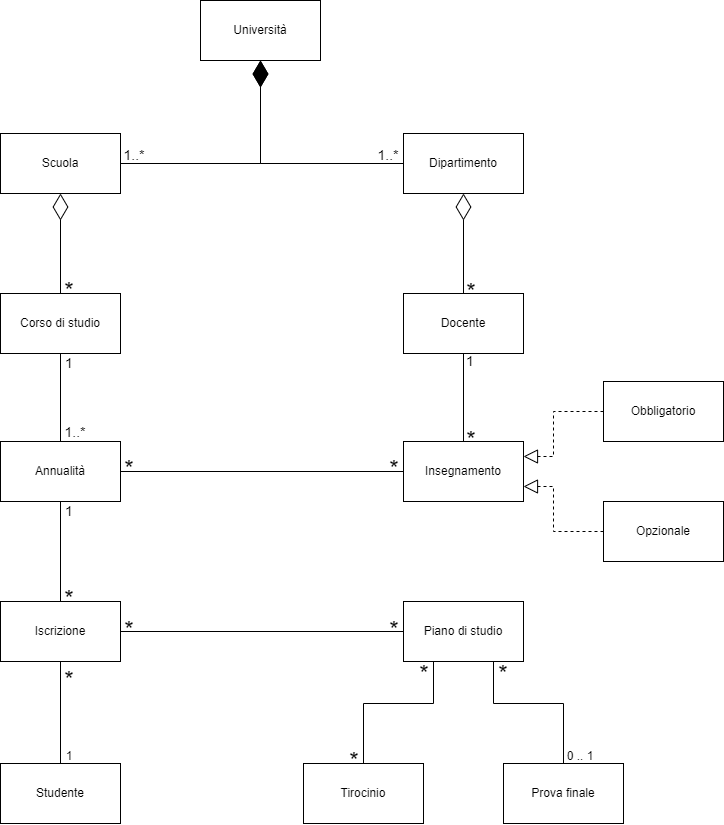
\includegraphics[width=1.05\textwidth]{foto 2.png}
\end{center}

\subsubsection*{Diagramma delle classi - post correzione}
\large
\vspace*{27pt}
\begin{center}
    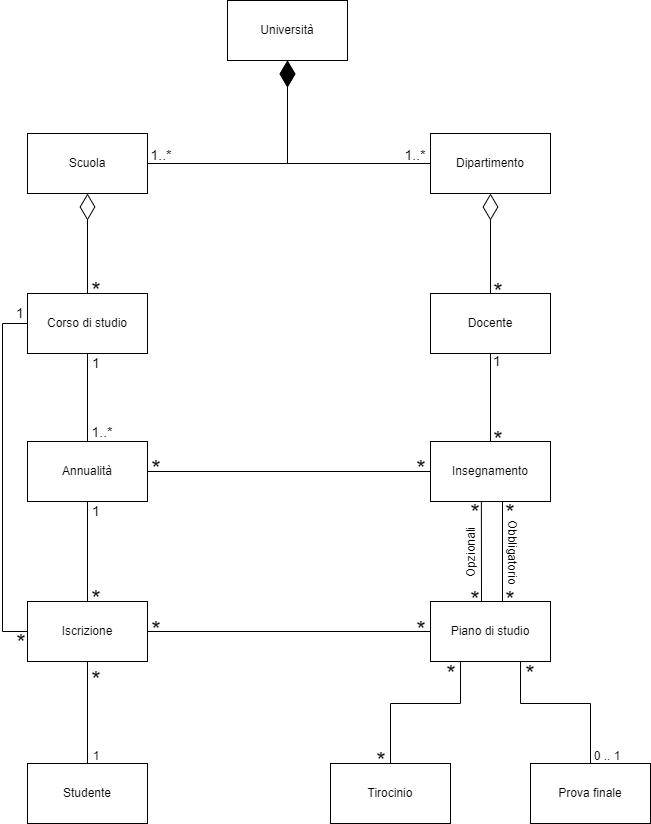
\includegraphics[width=1.02\textwidth]{foto 3.png}
\end{center}
\pagebreak
\subsubsection*{Considerazioni}
\large
\textit{Post correzioni}\\
In relazione a quanto descritto nella prima sezione, possono essere aggiunte ulteriori considerazioni.\vspace*{14pt}\\
Il primo passo della discussione ritrae nuovamente le associazoni utilizzate. E' bene indicare come una qualsiasi \textit{composizione} o \textit{aggregazione} pongano la cardinalità della classe, che compone o aggrega, ad \textit{1}; un esempio lampante è dato dalle classi \textit{Università} e \textit{Dipartimento}, dove un'università può contenere un numero indefinito di dipartimenti; tuttavia un dipartimento appartiene ad un unica università. Ciò si ripete per qualunque composizione e aggregazione del diagramma.\vspace*{14pt}\\
Proseguendo, si osserva una netta differenza tra \textit{Insegnamento} e \textit{Piano di studio}, in cui non sono più presenti le sottoclassi \textit{Opzionale} e \textit{Obbligatorio}. La ragione principale di questa variazione è dovuta ad un limite modellativo precedente, in quanto imponeva per un qualsiasi studente preso in considerazione, che i propri corsi si potessero distinguere in due singole opzioni, senza garantire l'imparzialità per successivi modelli adottati per nuovi elementi. Mediante la modifica apportata, è possibile garantire un atteggiamento specifico ed univoco nei confronti di ogni istanza della classe \textit{Studente}.\vspace*{14pt}\\
Concludendo, è buona pratica analizzare se sia possibile risalire ad informazioni inerenti ad istanze di qualche classe mediante il passaggio delle differenti associazioni. Tale effettività si riscontra qualora vi sia un dubbio in relazione al posizionamento di certi collegamenti tra i domini che costituiscono il diagramma. Da rappresentazione, si nota la nuova associazione posta tra le classi \textit{Iscrizione} e \textit{Corso di studio}; la ragione di tale scelta è causata dalla precedente impossibilità di poter risalire ad un unico corso di studio di uno studente. Infatti, la molteplicità (\textit{a molti}) non permette di usufruire delle medesime associazioni per recapitare i dati voluti, per cui l'uso di una connessione aggiuntiva ovvia a tale problema.
\end{document}